\chapter{Visualizing Data \cite{statistics/book/Statistics-for-Data-Scientists/Maurits-Kaptein}} \label{Visualizing Data}

\begin{enumerate}
    \item Visualization, when done well, can make large and even high-dimensional datasets (relatively) easy to interpret. \hfill \cite{statistics/book/Statistics-for-Data-Scientists/Maurits-Kaptein}

    
\end{enumerate}


\begin{lstlisting}[
    language=Python
]
import random
import faker                    # to generate fake data
import numpy as np
import pandas as pd
from tqdm import tqdm           # progress bar

# plotting libraries
import seaborn as sns           
import matplotlib.pyplot as plt

random.seed(0)
np.random.seed(0)
faker.Faker.seed(0)

fake = faker.Faker()
\end{lstlisting}


\section{Pairwise Plot \cite{statistics/book/Statistics-for-Data-Scientists/Maurits-Kaptein, data/online/seaborn.pairplot}} \label{Visualizing Data/Pairwise Plot}


\begin{table}[H]
\begin{minipage}[t]{0.35\linewidth}
\begin{figure}[H]
    \centering
    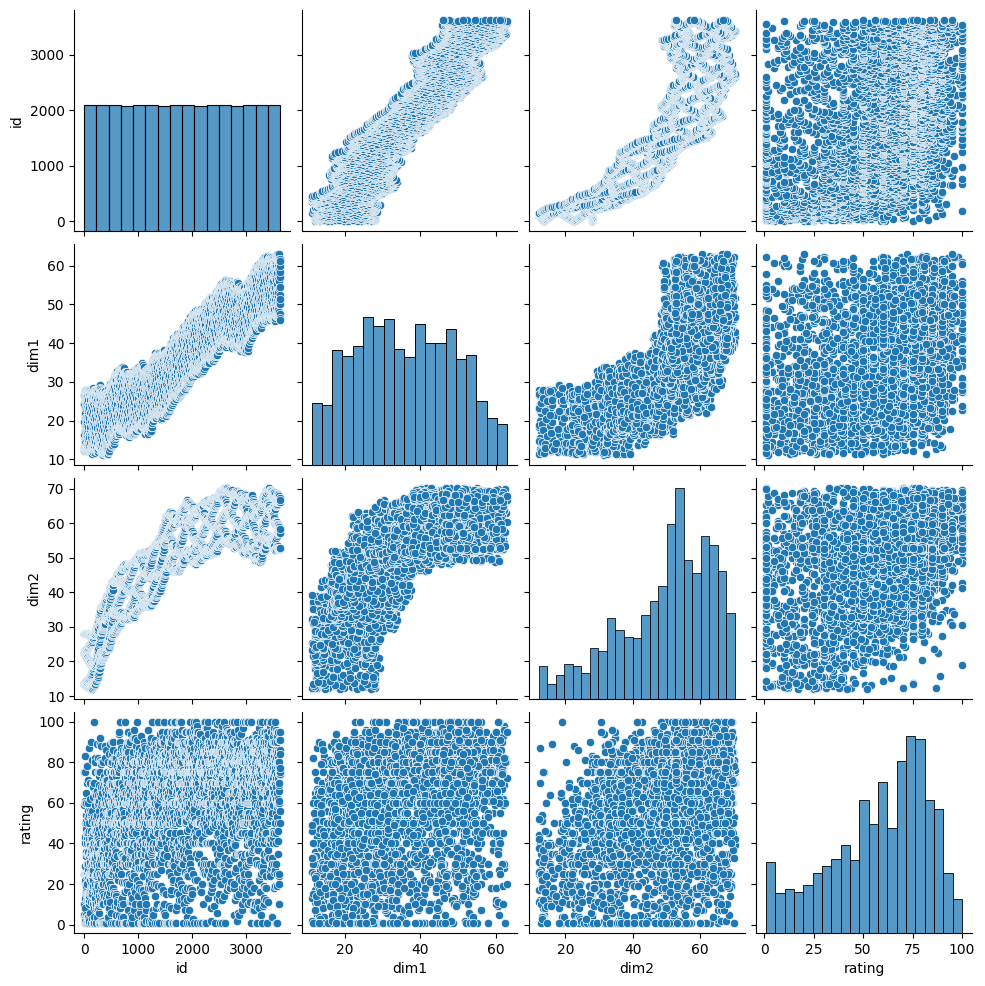
\includegraphics[width=0.9\linewidth, height=10cm, keepaspectratio]{images/data/__visualizations__/sns-pairplot-face-data.png}
    \caption{Pairwise plot (py-sns) output (face\_data.csv)}
\end{figure}
\end{minipage}
\hspace{0.2cm}
\vrule width 1pt
\hspace{0.5cm}
\begin{minipage}[t]{0.57\linewidth}
\begin{lstlisting}[
    language=Python,
    caption=Pairwise Plot: py-sns: face\_data.csv
]
df = pd.read_csv("face_data.csv")
sns.pairplot(df)
\end{lstlisting}

\vspace{0.3cm}

\begin{enumerate}
    \item Plot pairwise relationships in a dataset. \hfill \cite{data/online/seaborn.pairplot}

    \item By default, this is a grid of Axes such that each numeric variable in data will by shared across the y-axes across a single row and the x-axes across a single column. \hfill \cite{data/online/seaborn.pairplot}
    
    \item The diagonal plots are treated differently: a univariate distribution plot is drawn to show the marginal distribution of the data in each column. \hfill \cite{data/online/seaborn.pairplot}
\end{enumerate}
\end{minipage}
\end{table}










\section{Count Plot \cite{data/online/seaborn.countplot}} \label{Visualizing Data/Count Plot}


\begin{table}[H]
\begin{minipage}[t]{0.35\linewidth}
\begin{figure}[H]
    \centering
    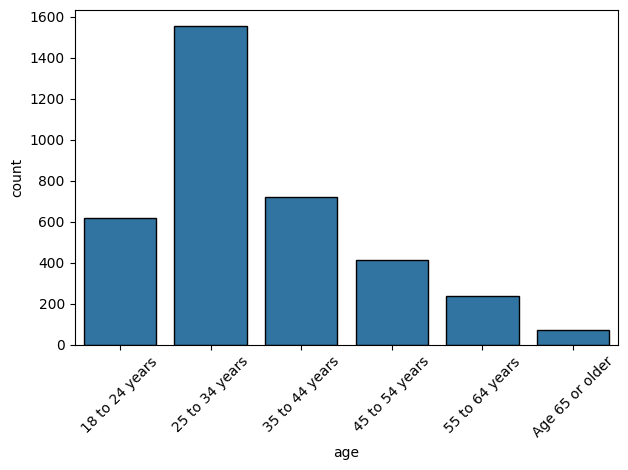
\includegraphics[width=0.9\linewidth, height=10cm, keepaspectratio]{images/data/__visualizations__/sns-countplot-face-data.png}
    \caption{Count plot (py-sns) output (face\_data.csv)}
\end{figure}
\end{minipage}
\hspace{0.2cm}
\vrule width 1pt
\hspace{0.5cm}
\begin{minipage}[t]{0.57\linewidth}
\begin{lstlisting}[
    language=Python,
    caption=Count Plot: py-sns: face\_data.csv
]
vals = df[df["age"] != " "].copy()

sns.countplot(
    x='age', 
    data=vals, 
    order=sorted(vals['age'].unique()), 
    edgecolor='black',
)

plt.xticks(rotation=45)
plt.tight_layout()
plt.show()
\end{lstlisting}
\end{minipage}
\end{table}

\vspace{0.3cm}

\begin{enumerate}
    \item Show the counts of observations in each categorical bin using bars.

    
\end{enumerate}

